%Ab hier können in den leeren, geschweiften Klammern die Informationen für das Deckblatt eintragen werden.
\newcommand{\praktikum}{} %Praktikum P3/P4:
\newcommand{\gruppennummer}{} %Gruppennummer:
\newcommand{\gruppentag}{} % Gruppentag (Mo1, Mo2, Mi3):
%Bitte zusätzlich den richtigen Wochentag, an dem ihr euer Praktikum absolviert, entkommentieren.
\newcommand{\gruppentagposition}{10cm,22.8cm} % Mo1 Gruppentag:
%\newcommand{\gruppentagposition}{11.7cm,22.8cm} % Mo2 Gruppentag:
%\newcommand{\gruppentagposition}{13.3cm,22.8cm} % Mi3 Gruppentag:
\newcommand{\semester}{} %Semester:
\newcommand{\versuch}{} %Versuch:
\newcommand{\nameeins}{} %Name1 (Vor und Nachname):
\newcommand{\emaileins}{} %E-Mail 1:
\newcommand{\namezwei}{} %Name2 (Vor und Nachname):
\newcommand{\emailzwei}{} %E-Mail 2:
\newcommand{\assistent}{} %Assistent*in:
\newcommand{\durchfuehrungsdatum}{} %Durchgeführt am:
\newcommand{\abgabedatum}{} %Protokollabgabe am:
%%%%%%%%%%%%%%%%%%%%%%%%%%%%%%%%%%%%%%%%%%%%%%%%%%%%%%%%%%%%%%%%%%%%%%%%%%%%%%%%%%%%%%%%%
%Ab hier gibt es nichts mehr auszufüllen.
\begin{tikzpicture}[remember picture,overlay]
    \node at (current page.center) {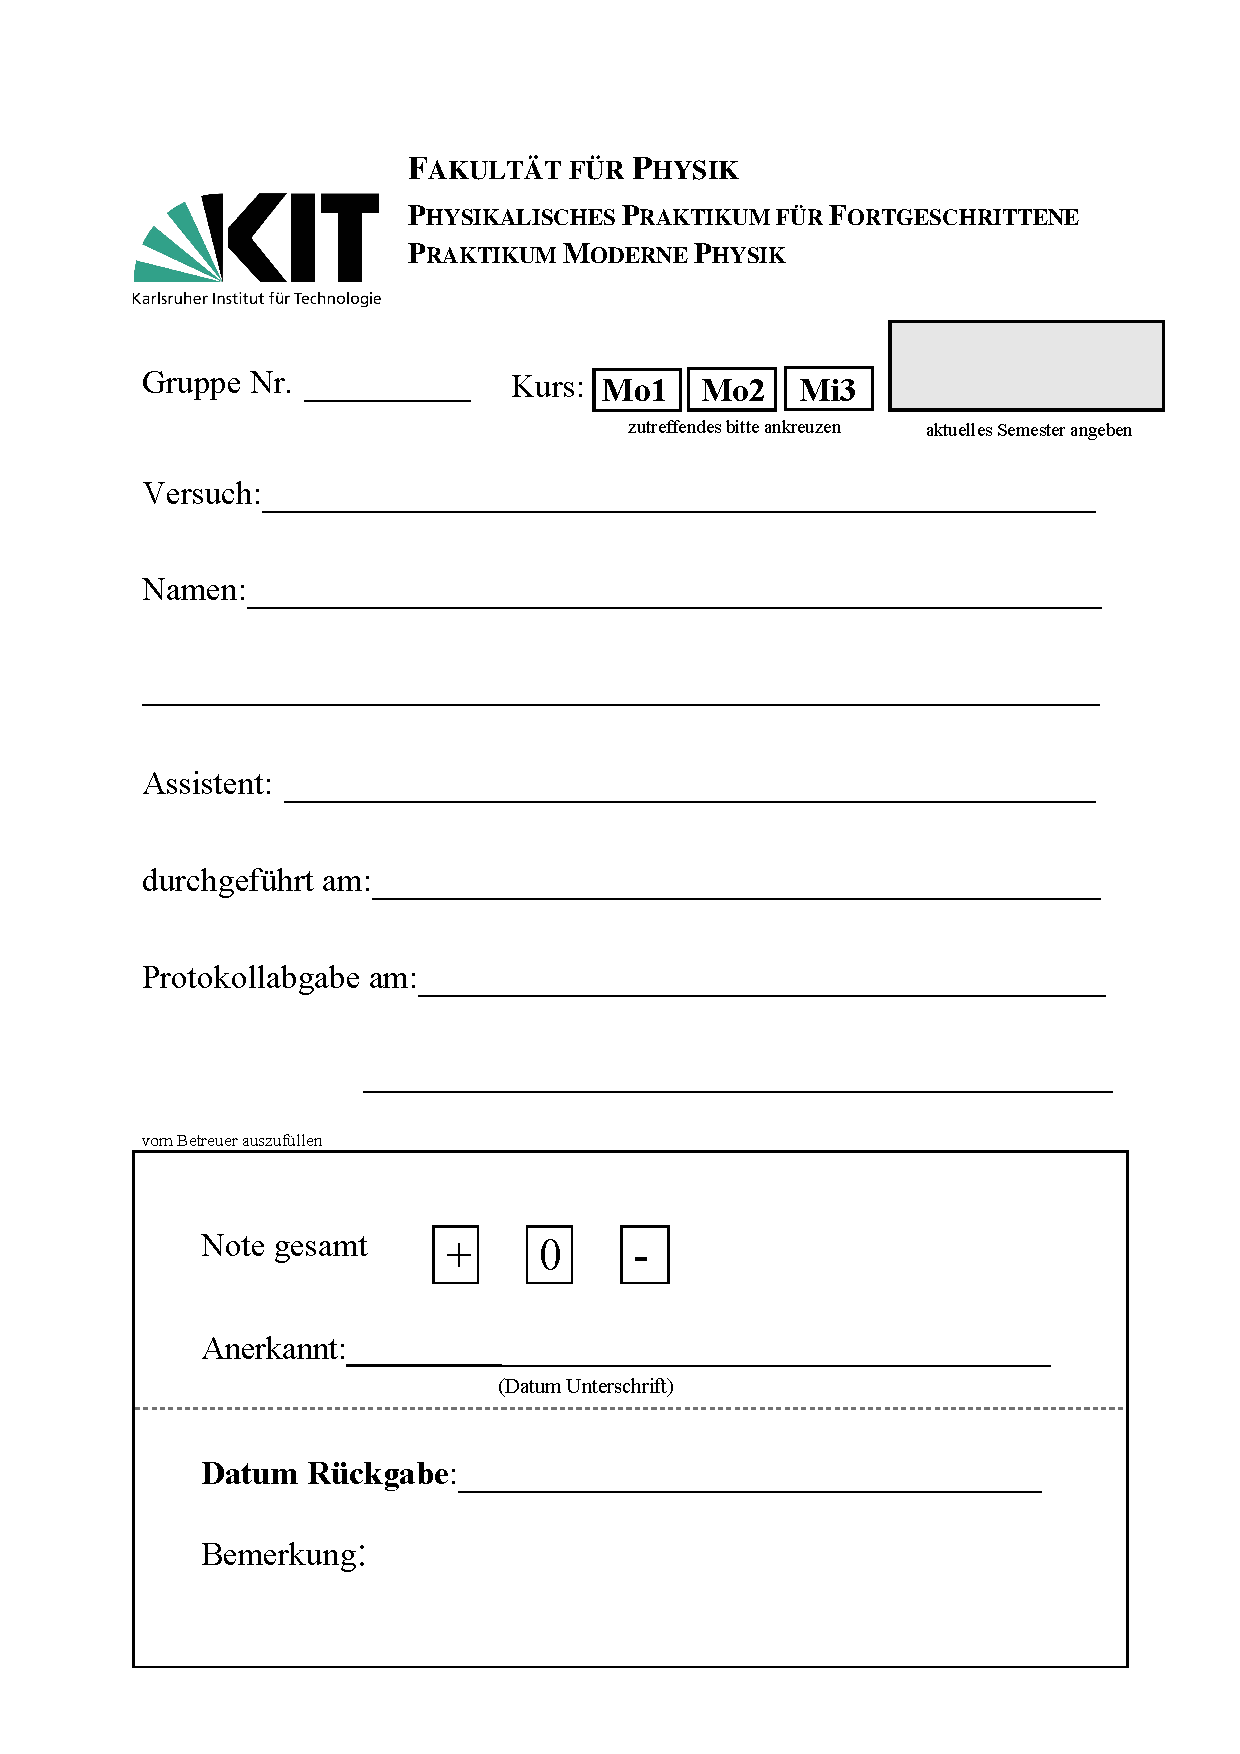
\includegraphics[page=1]{include/Deckblatt.pdf}};
    \begin{scope}[shift={(current page.south west)},every node/.style={anchor=base west}]
        \node at (5.8cm,23.1cm){\Large{\gruppennummer}};% Gruppennummer:
        \node at (\gruppentagposition) {\scalebox{4}{{$\mathbf{\times}$}}};% Gruppentag
        \node at (16cm,23.1cm) {\Large{\semester}}; % Semester:
        \node at (4.8cm,21.2cm){\Large{\versuch}}; %Versuch:
        \node at (4.8cm,19.6cm){\Large{\nameeins\hspace{0.2222em}(\emaileins)}}; % Name 1.Zeile:
        \node at (4.8cm,18.0cm){\Large{\namezwei\hspace{0.2222em}(\emailzwei)}}; % Name 2.Zeile:
        \node at (4.8cm,16.3cm){\Large{\assistent}}; % Assistent:in:
        \node at (7.2cm,14.6cm){\Large{\durchfuehrungsdatum}}; % durchgeführt am:
        \node at (7.2cm,13.0cm){\Large{\abgabedatum}}; % Protokollabgabe am:
    \end{scope}
\end{tikzpicture}
% Diese Informationen werden als Meta-Daten in die PDF-Datei eingebettet.
% Dabei werden die Informationen automatisch aus den eingetragenen Informationen übernommen.
\hypersetup{
  pdftitle    = {\praktikum\hspace{0.2222em}Protokoll - \versuch},
  pdfsubject  = {Protokoll des Versuchs \versuch\hspace{0.2222em}vom \durchfuehrungsdatum},
  pdfauthor   = {\nameeins\hspace{0.2222em}und\hspace{0.2222em}\namezwei\hspace{0.2222em}(Gruppe \gruppentag-\gruppennummer)},
  pdfkeywords = {KIT, Physik, Praktikum, Protokoll, \praktikum, \versuch, \semester, \nameeins, \namezwei},
  pdfcreator  = {pdflatex},
  pdfproducer = {LaTeX with hyperref}
}